Im \termlong{} wurde in Veranstaltungen der Fakultät für \facultylong{} eine Veranstaltungsevaluation durchgeführt. Dazu wurden die Studierenden in den Veranstaltungen gebeten, einen von der Fachschaft in Zusammenarbeit mit den Studienkommissionen sowie der Qualitätssicherungsabteilung der ZUV entworfenen Fragebogen auszufüllen. Deutsche und englische Fragebogenversionen unterscheiden sich einzig in der Sprache, damit auch Studierende ohne deutsche Sprachkenntnis die Möglichkeit haben, die Veranstaltung zu beurteilen. Den Studierenden wurde während der Veranstaltung Zeit zur Beurteilung der Veranstaltung und ggf. des Übungsbetriebs gegeben. Direkt im Anschluss daran wurden die Bögen wieder von Fachschaftsmitgliedern eingesammelt und anschließend ausgewertet.


\subsubsection{Erläuterungen zur Auswertung}

Speziell in Vorlesungen ohne Anwesenheitspflicht kann die Repräsentativität der Auswertung gering sein, wenn bereits viele die Veranstaltung nicht mehr besuchen. Dies lässt sich mit Hilfe
der Frage  „Ich schätze, dass im Vergleich zum Beginn der Vorlesung jetzt noch folgender Anteil der Studierenden teilnimmt“ beurteilen. Man kann annehmen, dass ein großer Anteil der AbbrecherInnen den Besuch wegen aus ihrer Sicht schlechter Präsentation des Vorlesungsstoffes oder ähnlichem aufgegeben hat. Davon abgesehen sollte die Anzahl der zurückgegebenen Fragebögen zur Einschätzung der Genauigkeit der Auswertung dienen. Bei einem zu geringen Rücklauf an Bögen je DozentIn oder TutorIn haben wir aus Gründen des Datenschutzes und der mangelnden Aussagekraft der Antworten keine Auswertung vorgenommen.



\subsubsection{Die Diagramme}

Die Histogramme hinter den Fragen entsprechen den Feldern auf den Fragebögen. Die Balkendiagramme geben die Häufigkeit wieder, mit der das entsprechende Feld angekreuzt wurde. Die Höhe der Balken ist dabei auf die Gesamtzahl von gültigen Stimmen ohne Enthaltungen normiert, die unter dem Fragetext vermerkt ist. Enthaltungen werden im Diagramm also \emph{nicht} berücksichtigt.

Die Mittelwertberechnung zu jeder Frage und Veranstaltung ergibt sich aus den jeweils gültigen Stimmen und ist durch den oberen (ausgefüllten) Punkt dargestellt. Der untere (unausgefüllte) Punkt stellt das Mittel über alle abgegebenen Bögen dar. Dabei wurden alle Bögen gleich gewichtet (kleinere Veranstaltungen fallen also schwächer ins Gewicht als große). Berücksichtigt wurden natürlich nur Bögen des aktuellen Semesters und der gleichen Fakultät. Der
jeweilige Balken gibt die Standardabweichung an.

Der Vergleich zwischen dem Mittelwert einer Veranstaltung und dem Gesamtmittel ist in vielen Fällen aussagekräftiger als der Absolutwert des Mittelwertes. Es sollte aber beachtet werden, dass sich die Veranstaltungen aufgrund zum Teil völlig unterschiedlicher Situationen manchmal nicht vergleichen lassen.

\subsubsection{Beispiele}
\begin{tikzpicture}
\globalQuestion{
  Mein Lernzuwachs ist hoch.\\
  {\globalNumberStyle
    Antworten: 7,
    Enthaltungen: 0}
}
\singleHistogramPoleLeft{stimme voll zu}
\singleHistogramHist{14,57,29,0,0}
\singleHistogramErr{2.1429}{0.6389}[3.9951][1.0779]
\singleHistogramPoleRight{stimme gar nicht zu}


\node at (0.8, 2.2) [text width = 8cm, text ragged left]
  {\footnotesize rechter Pol};
\draw (5,2.2) .. controls (12.2,2.2) .. (12.2,0.6);

\node at (0.8, 1.7) [text width = 8cm, text ragged left]
  {\footnotesize relative Häufigkeit der \emph{Antworten} und Histogramm};
\draw[decorate,decoration=brace] (5.9,0.9) -- (11.3,0.9);
\draw (5,1.7) .. controls (8.6,1.7) .. (8.6,0.995);

\node at (0.8, 1.2) [text width = 8cm, text ragged left]
  {\footnotesize linker Pol};
\draw (5,1.2) .. controls (5.4,1.2) .. (5.4,0.5);


\node at (0.8, -1.7) [text width = 8cm, text ragged left]
  {\footnotesize Mittelwert und Standardabw. \emph{dieser} Veranstaltung};
\draw (5,-1.7) .. controls (7.7,-1.7) .. (7.7,-0.9);

\node at (0.8, -2.2) [text width = 8cm, text ragged left]
  {\footnotesize Mittelwert und Standardabw. \emph{aller} Veranstaltungen};
\draw (5,-2.2) .. controls (9.65,-2.2) .. (9.65,-1.05);
\end{tikzpicture}

\vspace*{1cm}

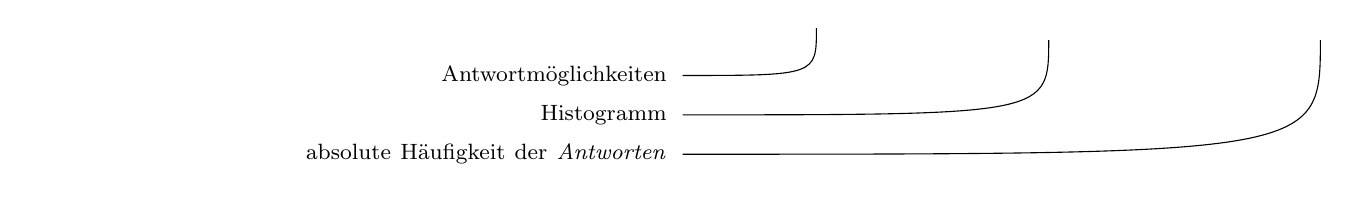
\begin{tikzpicture}
\globalQuestion{
  Mit welchem \emph{Abschlussziel} studierst Du?\\
  {\globalNumberStyle
    Antworten: 7,
    Enthaltungen: 0}
}

\singleHorizontalBars{Bachelor,Master}{1,6}

\node at (0.8, -1.5) [text width = 8cm, text ragged left]
  {\footnotesize Antwortmöglichkeiten};
\draw (5,-1.5) .. controls (6.7,-1.5) .. (6.7,-0.9);

\node at (0.8, -2.0) [text width = 8cm, text ragged left]
  {\footnotesize Histogramm};
\draw (5,-2.0) .. controls (9.65,-2.0) .. (9.65,-1.05);

\node at (0.8, -2.5) [text width = 8cm, text ragged left]
  {\footnotesize absolute Häufigkeit der \emph{Antworten}};
\draw (5,-2.5) .. controls (13.1,-2.5) .. (13.1,-1.05);
\end{tikzpicture}



\subsubsection{Zu den Kommentaren}

An der ungekürzten Übernahme von Kommentaren zu einer Veranstaltung wurde kritisiert, dass so einzelne Meinungen in krassem Missverhältnis zur Statistik aller Studierenden überbewertet würden. Wir gingen daher zwischenzeitlich dazu über, Statistik und Kommentare zu sichten und gaben ein Gesamtbild der Veranstaltung in der Zusammenfassung an. Mittlerweile hat sich die Stimmung geändert und viele DozentInnen sind der Ansicht, dass das unverfälschte Übernehmen der Kommentare die bessere Alternative sei. Die Kommentare zu einer Veranstaltung werden deshalb wieder abgetippt und sind im Verhältnis zur gesamten HörerInnenzahl zu betrachten.


\subsubsection{Allgemeine Bemerkungen zur Beurteilung der Lehrveranstaltungen}

Die Mittelwerte über alle Veranstaltungen liegen meist höher als die neutralen Werte. Die Veranstaltungen scheinen von den Studierenden geringfügig besser als eine durchschnittliche Veranstaltung empfunden zu werden. Die Evaluation soll dazu dienen, Anhaltspunkte für die Verbesserung der Lehre zu geben. Sie ist von den DozentInnen und TutorInnen als konstruktive Kritik zu sehen. Die Aussagekraft und Notwendigkeit dieses studentischen Meinungsbildes sollte von allen Fakultätsmitgliedern anerkannt werden.

\subsubsection{Verfügbarkeit der Evaluation}

Diese Evaluation ist üblicherweise für ein Semester an den verschiedenen Aushängeorten zu finden und kann darüber hinaus durch Anfrage im Fachschaftsraum eingesehen werden.

Die Evaluation der Fakultät für Mathematik und Informatik ist zusätzlich aus dem internen Netz der Universität oder mittels VPN als PDF-Dokument verfügbar:

\url{http://mathphys.fsk.uni-heidelberg.de/evaluation.html}
